\section{Análise Bivariada}

\hrulefill

\hrulefill



\subsection{Registros}

\begin{resposta}
Os valores de correlação, valor-p e número de municípios encontram-se na tabela a seguir:
\end{resposta}


\begin{figure}[h!]
\centering
{\scriptsize Tabela 10. Correlação linear entre o número de registros (Log10) por município em cada banco de dados e variáveis explanatórias. WAV = Wikiaves, SLI = SpeciesLink, WAV2 = WAV com municípios redundantes em SLI. Número de municípios (n), coeficiente de correlação de Pearson (r) para cada pareamento, com outliers bivariados excluídos. Valores significantes $(p < 0.05)$ em negrito. }
\\
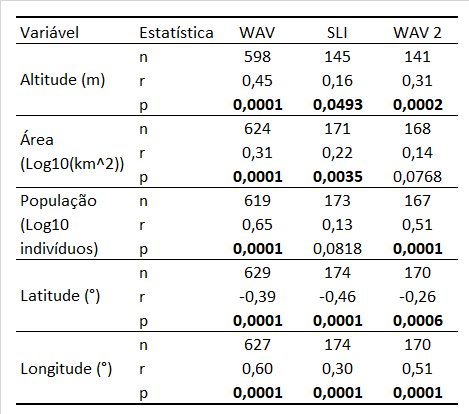
\includegraphics{Imagens/T10.png}
\end{figure}

 

\subsubsection{Altitude}

\begin{figure}[h!]
\centering
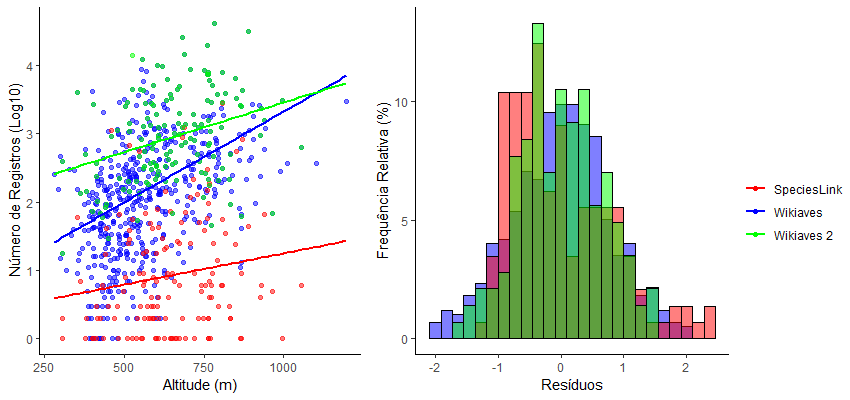
\includegraphics[width = 15cm]{Imagens/G01.png}
\\{\scriptsize Figura 9. Relação linear entre o número de registros (Log10) em cada banco de dados e a altitude (m) da sede dos municípios (esquerda) e respectiva distribuição de resíduos (direita, em unidades de desvio-padrão, em unidades de desvio-padrão). Outliers bivariados foram excluídos. }
\end{figure}
\newpage

\begin{resposta}
Para o estado de São Paulo, embora hajam valores baixos de $p$ para o Wikiaves, o espaço amostral é de 598 municípios, portanto, espera-se que estes valores sejam pequenos. Para o SpeciesLink, a medida de $p$ que é maior que $0,01$, está próxima a este valor. O gráfico abaixo servirá de indicativo para determinar se a evidência coletada é o suficiente para a rejeição da hipótese nula.

De fato, a quantidade de registros no Wikiaves aumenta conforme o aumento de altitude. Contudo, não é um aumento evidente, há muitos pares ordenados distantes da reta, isto é, a reta de regressão neste caso não é uma boa aproximação para esta curva. Para o SpeciesLink, os gráficos explicitam que o valor de $p < 0,05$ e próximo a $0,01$ não é o suficiente para a rejeição da hipótese nula, na verdade, os dados mostram-se distantes da reta e sem padrão definido.

Quanto aos municípios registrados em ambos os bancos de dados, percebe-se, no Wikiaves, um aumento relevante do valor de $p$, que pode ser explicado pela diminuição da quantidade de cidades. 
\end{resposta}



\subsubsection{Área}


\begin{figure}[h!]
\centering
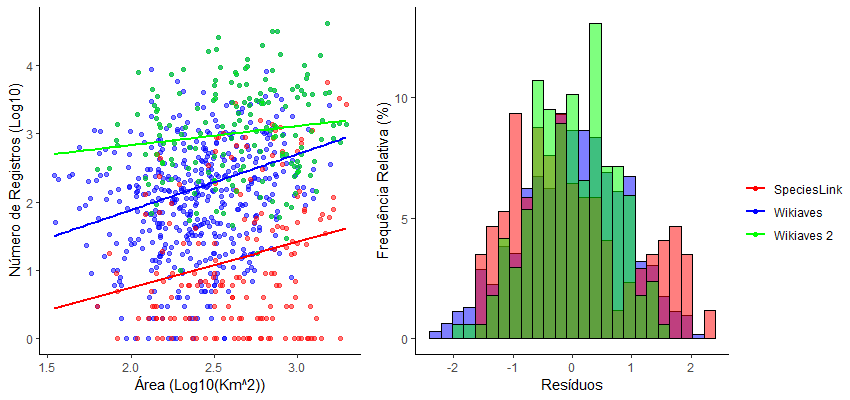
\includegraphics[width = 15cm]{Imagens/G02.png}
\\{\scriptsize Figura 10. Relação linear entre o número de registros (Log10) em cada banco de dados e a área (Log10 km2) dos municípios (esquerda) e respectiva distribuição de resíduos (direita, em unidades de desvio-padrão). Outliers bivariados foram excluídos.}
\end{figure}

\begin{resposta}
 Os valores de correlação linear para os municípios registrados no Wikiaves ou no SpeciesLink são de $0,31$ e $0,22$, respectivamente. Devido aos baixos valores de $p$ é possível que haja uma correlação não linear entre o que analisando, para confirmar ou contestar isto, atente-se ao gráfico: 
 
 É relevante que não há outliers bivariados. Além disto, há, de fato, um aumento linear, apesar disto, os pares ordenados encontram-se dispersos da reta de regressão, o que explica os baixos valores de correlação.

Ao diminuir a quantidade de cidades no Wikiaves, os valores de $p$ aumentam, torna-se maior que $0,01$, seguidos de valores baixos de $r$ em ambos. 

De fato, é possível afirmar que este parâmetro não possui grande influência sobre a quantidade de registros nas duas bases.
\end{resposta}



\subsubsection{População}

\begin{figure}[h!]
\centering
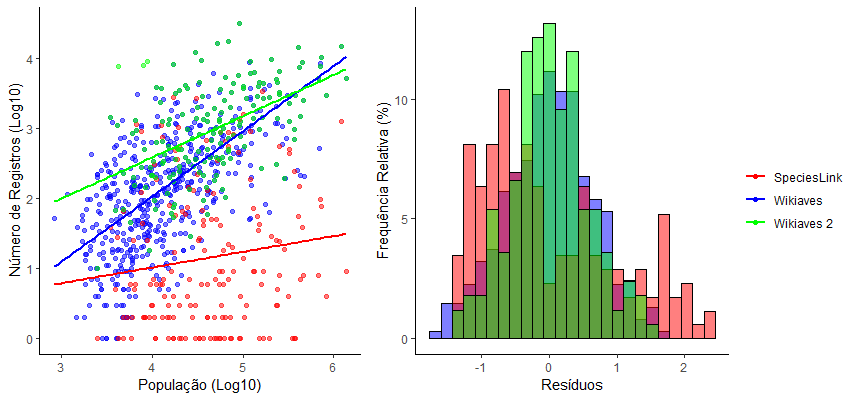
\includegraphics[width = 15cm]{Imagens/G03.png}
\\{\scriptsize Figura 11. Relação linear entre o número de registros (Log10) em cada banco de dados e o tamanho da população humana (Log10 indivíduos) dos municípios (esquerda) e respectiva distribuição de resíduos (direita, em unidades de desvio-padrão). Outliers bivariados foram excluídos.}
\end{figure}

\begin{resposta}
 O valor de correlação para os 619 municípios analisados para o Wikiaves é o maior obtido até então: $0,65$, um forte indicativo que há correlação linear nesta base. Em contrapartida, o SpeciesLink apresenta $p = 0,08$, que é um valor que exige cautela, como a correlação nesta base é de $0,13$ é possível assumir que não há correlação linear. Os gráficos a seguir confirmam isto.
 
\end{resposta}

\subsubsection{Latitude}

\begin{figure}[h!]
\centering
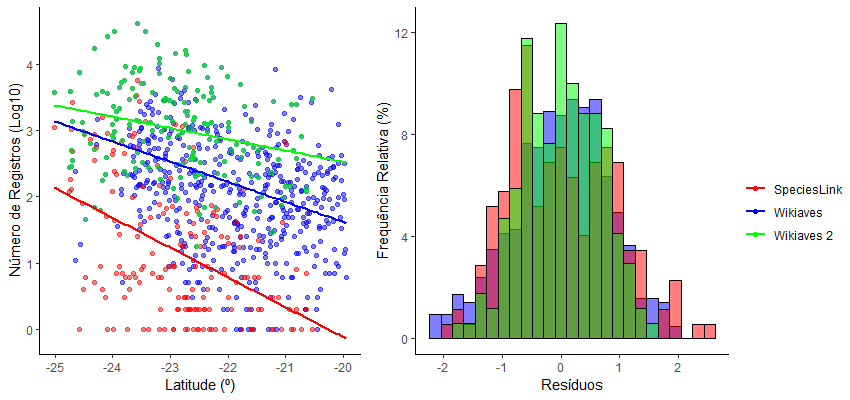
\includegraphics[width = 15cm]{Imagens/G04.png}
\\{\scriptsize Figura 12. Relação linear entre o número de registros (Log10) em cada banco de dados e a latitude (graus) da sede dos municípios (esquerda) e respectiva distribuição de resíduos (direita, em unidades de desvio-padrão). Outliers bivariados foram excluídos.}
\end{figure}

\newpage

\begin{resposta}
 Os valores de $p$ e $r$, aparentam ser o suficiente para constatar que há um decaimento na quantidade de registros conforme aumento de altitude. 
 
 Os resíduos são regulares ao passo que estão dispersos da reta de regressão, há correlação linear, porém é baixa. Ao retirar as cidades excedentes os valores aumentam (no caso, o relacionamento é menor) no Wikiaves.
\end{resposta}

\subsubsection{Longitude}

\begin{figure}[h!]
\centering
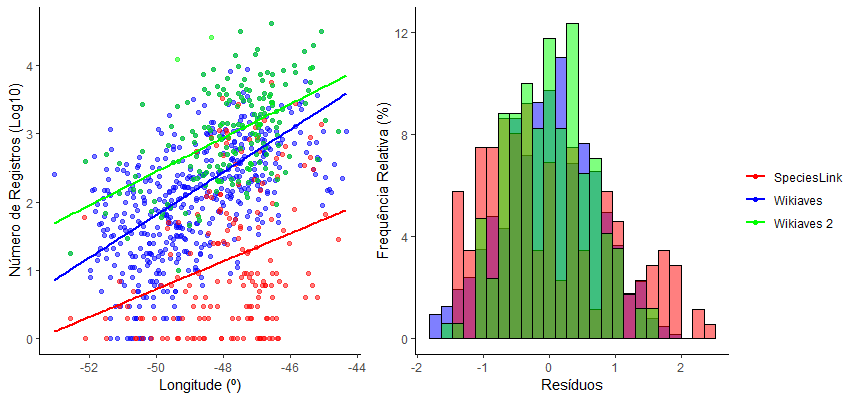
\includegraphics[width = 15cm]{Imagens/G05.png}
\\{\scriptsize Figura 13. Relação linear entre o número de registros (Log10) em cada banco de dados e a longitude (graus) da sede dos municípios (esquerda) e respectiva distribuição de resíduos (direita, em unidades de desvio-padrão). Outliers bivariados foram excluídos.}
\end{figure}

 \begin{resposta}
O aumento linear é claro no Wikiaves e, embora não seja tão evidente assim, há um aumento no SpeciesLink, também.

Os resíduos regulares, bem como, o aumento no gráfico indicam que há relação.
\end{resposta}


\subsection{Espécies}

\begin{resposta}
Os valores de correlação, valor-p e número de municípios encontram-se na tabela a seguir:
\end{resposta}

\newpage

\begin{figure}[h!]
\centering
{\scriptsize Tabela 11: Correlação linear entre o número de espécies (Log10) por município em cada banco de dados e variáveis explanatórias. WAV = Wikiaves, SLI = SpeciesLink, WAV2 = WAV com municípios redundantes em SLI. Número de municípios (n), coeficiente de correlação de Pearson (r) para cada pareamento, com outliers bivariados excluídos. Valores significantes $(p < 0.05)$ em negrito.}
\\
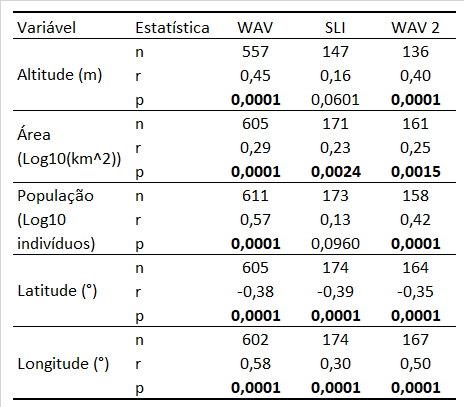
\includegraphics{Imagens/T11.png}
\end{figure}

\subsubsection{Altitude}


 

\begin{figure}[h!]
\centering
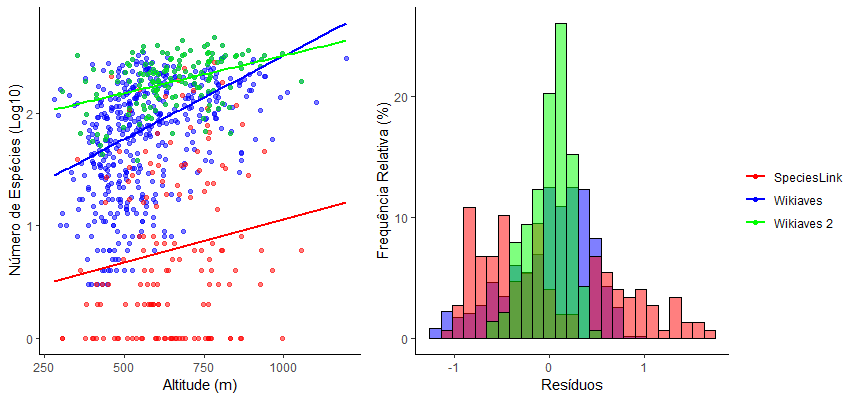
\includegraphics[width = 15cm]{Imagens/G06.png}
\\{\scriptsize Figura 14: Relação linear entre o número de espécies (Log10) em cada banco de dados e a altitude (m) da sede dos municípios (esquerda) e respectiva distribuição de resíduos (direita, em unidades de desvio-padrão). Outliers bivariados foram excluídos.}
\end{figure}


\begin{resposta}
Os valores de $p$ para a quantidade de espécies são, ainda, maiores que os que dizem respeito aos registros, neste cenário, é possível assumir que não há relação entre a altitude e os dados do SpeciesLink ($p > 0,05$). No caso da outra base, os valores de $p$ são baixos o suficiente para que haja relação. O gráfico abaixo explicita o comportamento. Novamente, os dados estão dispersos da linha de tendência no Wikiaves. No SpeciesLink, de fato, não há correlação linear.

Ao admitir apenas os 173 municípios registrados por ambas as bases, o valor de $p$ para o Wikiaves não sofre uma mudança tão drástica quanto para os registros, na verdade, este valor continua abaixo de $0,01$. Note, no gráfico abaixo, que os valores não estão dispersos da linha de tendência, portanto, pode assumir que há uma relação.
\end{resposta}

\subsubsection{Área}



\begin{figure}[h!]
\centering
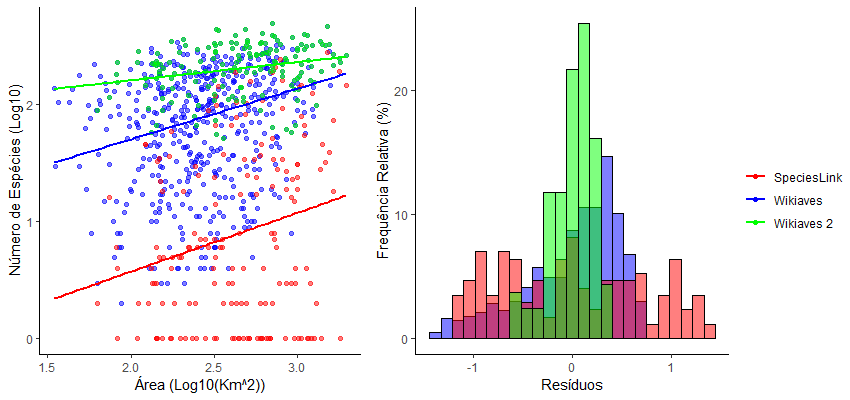
\includegraphics[width = 15cm]{Imagens/G07.png}
\\{\scriptsize Figura 15: Relação linear entre o número de espécies (Log10) em cada banco de dados e a área (Log10 km2) dos municípios (esquerda) e respectiva distribuição de resíduos (direita, em unidades de desvio-padrão). Outliers bivariados foram excluídos.}
\end{figure}

 \begin{resposta}
Quanto a quantidade de espécies os valores de $r$ diminuem no Wikiaves e aumentam no SpeciesLink, entretanto, não o suficiente para concluir que há ou não correlação linear entre as variáveis.

Tanto pelo gráfico quanto pelo modo com o qual os resíduos estão distribuídos identifica-se que não há correlação linear entre os dados. A situação não se altera ao se retirar os municípios excedentes. No geral, o tamanho de um município não possui grande influência em relação as variáveis resposta.
\end{resposta}

\subsubsection{População}

 \newpage

\begin{figure}[h!]
\centering
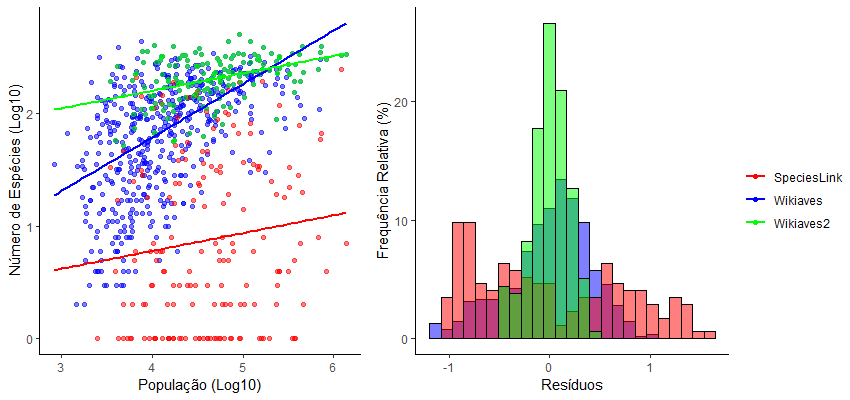
\includegraphics[width = 15cm]{Imagens/G08.png}
\\{\scriptsize Figura 16: Relação linear entre o número de espécies (Log10) em cada banco de dados e o tamanho da população humana (Log10 indivíduos) dos municípios (esquerda) e respectiva distribuição de resíduos (direita, em unidades de desvio-padrão). Outliers bivariados foram excluídos.}
\end{figure}

\begin{resposta}
De forma semelhante aos registros, a quantidade de espécies parece seguir o mesmo padrão. O valor de correlação é menor, percebe-se pelo gráfico que há relação para o Wikiaves. De fato, há um crescimento no Wikiaves, vez que, o SpeciesLink não segue padrão algum. Ao retirar os municípios excedentes o coeficiente angular da reta do Wikiaves aproxima-se de 0, ainda, é possível observar a relação.

Conclui-se que, este parâmetro influencia o Wikiaves, apenas. Ou seja, as bases de dados divergem quanto ao comportamento analisado nesta seção.
\end{resposta}

\subsubsection{Latitude}

 

\begin{figure}[h!]
\centering
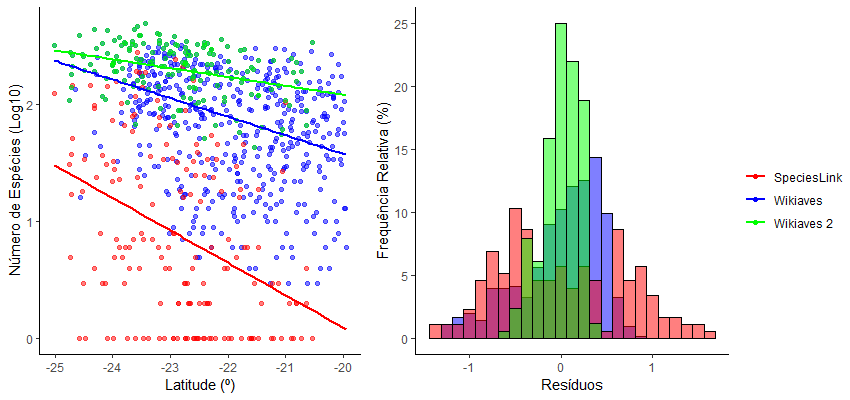
\includegraphics[width = 15cm]{Imagens/G09.png}
\\{\scriptsize Figura 17: Relação linear entre o número de espécies (Log10) em cada banco de dados e a latitude (graus) da sede dos municípios (esquerda) e respectiva distribuição de resíduos (direita, em unidades de desvio-padrão). Outliers bivariados foram excluídos.}
\end{figure}

\begin{resposta}
Para a quantidade de espécies os bancos de dados apresentam valores próximos de $r$. Note o comportamento nos gráficos:

O valor dos resíduos no Wikiaves aumentam conforme aumento da altitude e, no SpeciesLink, ocorre o oposto. No geral, assume-se uma correlação fraca entre este fator e a quantidade de espécies. De fato, o mesmo vale para quando se retira os municípios com registro em apenas uma das bases.
\end{resposta}

\subsubsection{Longitude}

\begin{figure}[h!]
\centering
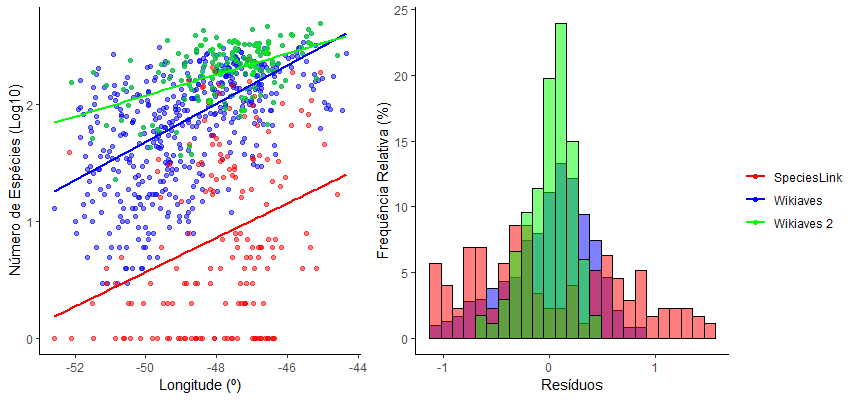
\includegraphics[width = 15cm]{Imagens/G10.png}
\\{\scriptsize Figura 18: Relação linear entre o número de espécies (Log10) em cada banco de dados e a longitude (graus) da sede dos municípios (esquerda) e respectiva distribuição de resíduos (direita, em unidades de desvio-padrão). Outliers bivariados foram excluídos.}
\end{figure}

 \begin{resposta}
Novamente, os pares ordenados estão dispersos da linha de tendência, contudo, os quartis regulares e o crescimento são indícios de que há relação. Isso se mantém ao retirar os municípios com registro em apenas uma das bases.
\end{resposta}
